\section{Datos originales}
El conjunto de datos encrudo son archivos en formato xlsx, desde el 2020 hasta el 2024, 
donde se tiene el reporte por hora de: 
\begin{itemize}
    \item Energ\'ia Activa Consumo (kWh).
    \item Energ\'ia Activa Generaci\'on (kWh).
    \item Energ\'ia Reactiva Inductiva (kVarh).
    \item Energ\'ia Reactiva Capacitiva (kVarh).
    \item Fecha.
\end{itemize}

Se presentan unos datos at\'ipicos enero de 2021 a junio 2021, esplicados por paros, apagones en la empresa.
Debido a que est\'as anomalias son provocadas por sucesos ajenos a un error en la c\'odificaci\'on del dato, no se procede a 
eliminarlos, ya que son datos reales y pueden afectar el modelo.

Al conjunto de datos se hace una limpieza y agrupaci\'on en un solo archivo permitiendonos tener un conjunto de datos con una ventana de tiempo de 
febrero de 2020 a septiembre de 2024. Con la siguente estructura de datos:
\begin{table}[h!]
    \centering
    \caption{Muestra de datos de energ\'ia }
    \hspace{0.01cm}
    \resizebox{\linewidth}{!}{ % Ajusta la tabla al ancho del documento
        \begin{tabular}{|c|c|c|c|c|}
        \hline
         \textbf{Fecha} &     \textbf{Activa Consumo} & \textbf{Activa Generaci\'on} & \textbf{Reactiva Capacitiva} & \textbf{Reactiva Inductiva}  \\ \hline
         2020-02-16     & 4948.0                      & 0.0                          & 0.0                          & 1382.0                             \\ \hline
         2020-02-17     & 14400.0                     & 0.0                          & 0.0                          & 7072.0                             \\ \hline
         2020-02-18     & 14896.0                     & 0.0                          & 0.0                          & 7640.0                             \\ \hline
         2020-02-19     & 14976.0                     & 0.0                          & 0.0                          & 7800.0                             \\ \hline
         2020-02-20     & 16104.0                     & 0.0                          & 0.0                          & 8376.0                             \\ \hline
        \end{tabular}
    }
    
    \label{tabla:tabla_energia}
    \end{table}
    En la tabla podemos \cite{tabla_energia} 
    En la siguiente gr\'afica tenemos los datos originales gr\'aficados    
      \begin{figure}[h!]
        \centering
        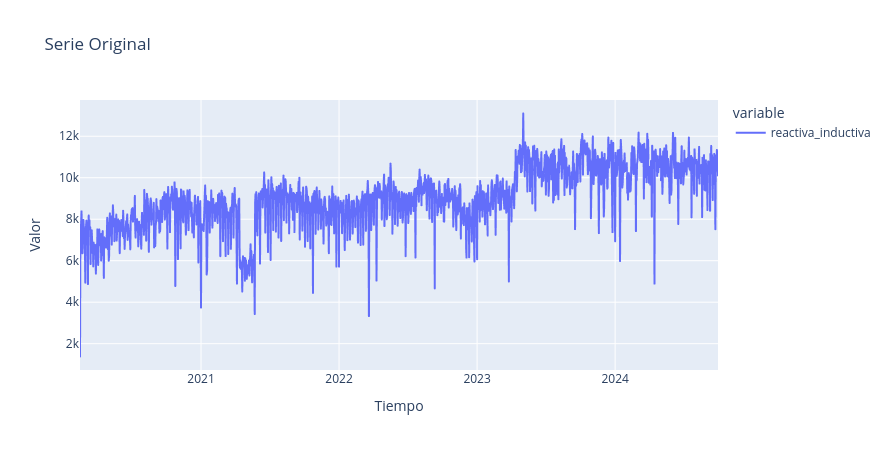
\includegraphics[width=0.8\textwidth]{/home/javier/Documentos/Javier/MiPregradoDeVida/Postgrado/especializacion/monografia/LaTex/images/newplot.png} % Cambia "ruta/de/la/imagen.jpg" por el nombre de tu archivo
        \caption{Energ\'ia reactiva}
        \label{fig:energia_reactiva_original}
    \end{figure}


\begin{filecontents}{data.dat}
  x y
  0 0.2
  1 3.3
  2 1.5
  3 1.1
  4 2.5
  \end{filecontents}

% \begin{figure}[h!]
%     \centering
%     \resizebox{\linewidth}{!}{ % Ajusta la tabla al ancho del documento
%             \begin{tikzpicture}
%                 % Cuadrícula de referencia
%                 \draw[very thin,color=gray] (-0.5,-1) grid (6.5,10);
%                 % Ejes x e y
%                 \draw[->] (-0.5,0) -- (7,0) node[right] {$x$};
%                 \draw[->] (0,-1) -- (0,6) node[above] {$y$};
%                 % Conjunto de puntos con fechas en el eje x
%                 \draw[color=blue, thick] plot coordinates {(1,2) (2,3.5) (3,4) (4,3) (5,15)};
%                 % Etiquetas para las fechas en el eje x
%                 \node[below] at (1,0) {2024-01-01};
%                 \node[below] at (2,0) {2024-02-01};
%                 \node[below] at (3,0) {2024-03-01};
%                 \node[below] at (4,0) {2024-04-01};
%                 \node[below] at (5,0) {2024-05-01};
%                 % Etiqueta de la curva
%                 \node[above] at (5,5) {Curva de ejemplo};
%             \end{tikzpicture}
%     }
%         \caption{Gr\'afico}
%         \label{fig:ejemplo}
% \end{figure}
\begin{tikzpicture}
  \begin{axis}
      \addplot table {data.dat};
  \end{axis}
\end{tikzpicture}

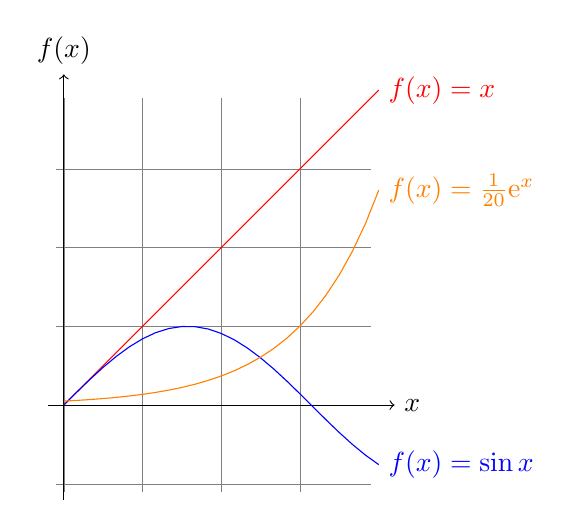
\begin{tikzpicture}[domain=0:4]
    \draw[very thin,color=gray] (-0.1,-1.1) grid (3.9,3.9);      
    \draw[->] (-0.2,0) -- (4.2,0) node[right] {$x$};
    \draw[->] (0,-1.2) -- (0,4.2) node[above] {$f(x)$};      
    \draw[color=red]    plot (\x,\x)             node[right] {$f(x) =x$};
    % \x r means to convert '\x' from degrees to _r_adians:
    \draw[color=blue]   plot (\x,{sin(\x r)})    node[right] {$f(x) = \sin x$};
    \draw[color=orange] plot (\x,{0.05*exp(\x)}) node[right] {$f(x) = \frac{1}{20} \mathrm e^x$};
\end{tikzpicture}
